\section{Autocrop Results}
\label{sec:autocropResults}

For the improved auto cropping mechanism there are many different versions implemented in this work.
All of them have been evaluated on the Switch evaluation dataset.
Even though the cropping mechanism is primarily designed for the inference of videos, performance differences can be recorded in this dataset.
The track of each image is predicted 50 times and the crop coordinates are adjusted iteratively.
The Results of autocrop versions are shown in \autoref{tab:autocropResults}.

\begin{table}[H]
    \centering
    \begin{tabular}{|l|c|c|c|c|c|}
    %\begin{tabular}{| p{0.3\linewidth} | p{0.6\linewidth} |}
        \hline
        \textbf{used Methods} & \textbf{original \cite{tepNet2024}} & \textbf{Version 2} & \textbf{Version 3} & \textbf{Version 4} & \textbf{Version 5}\\
        \hline
        RA                                 & \checkmark &            &            &            &            \\
        \hline
        EMA                                &            & \checkmark & \checkmark & \checkmark & \checkmark \\
        \hline
        reset rule [40\%] $(\frac{1}{3}, \frac{1}{2}, \frac{2}{3})$  &            & \checkmark & \checkmark & \checkmark & \checkmark \\
        \hline
        aspect ratio (16:9)   	           &            &            & \checkmark &            &            \\
        \hline
        aspect ratio (1:1)                 &            &            &            & \checkmark &            \\
        \hline
        10\% at the start                  &            &            &            &            & \checkmark \\
        \hline
        Switch evaluation dataset          & 88.97\%    & \textbf{91.18\%} & 86.76\% & 91.18\% & 90.44\%    \\
        \hline
    \end{tabular}
    \caption{Various versions of autocrops evaluated on the Switch evaluation dataset.
    Models predict each image 50 times and adjust the autocrop iteratively.
    Version 2 includes multiple experiments different parameters for the reset rule.
    Since the Evalutation dataset consists of images and the reset rule is applied in video sequences, only the best-performing parameters are included in this table.}
    \label{tab:autocropResults}
\end{table}

An improvement in accuracy can be observed in all versions but version 3.
In Version 3, the crop is forced to be in a 16:9 aspect ratio.
It is assumed that this ratio presents a disadvantage since the crop is resized in a quadratic 512 $\times$ 512 image afterward.
This assumption is supported by Version 4 also achieving the highest score.
This version has a fixed quadratic aspect ratio.

Version 5 is very similar to Version 2 but instead of starting with the whole image, its initial crop coordinates are set to $(0, 0.1 \times image\_height, 1)$.
The whole image width but only the lowest 10\% of the image are considered.
This proves to be effective in some cases, resulting in a much quicker convergence to a desired crop.
However, it also shows that it is highly situational dependent.
Version 5 works better than starting with the whole image only when a single track is visible in the beginning.
In starting scenarios with at least two tracks the model struggles to find the right one. Therefore the use of Version 5 is not recommended.
Version 2 and 4 are the highest-performing methods.
However, for this work Version 2 is used for further experiments because it does not introduce additional heuristics like Version 4.
Therefore, it is more independent of scene situations.

The parameters of the reset rule, such as the allowed percentage by which the prediction can descend and the crop coordinates to which the crop is reset, are determined based on the observed behavior of the models in various scenarios.
These parameters are described in \autoref{sec:autocropExperiments} in more detail.
In uncertainty, all Models have receding horizon lines, even though different backbones are used.
Therefore the crop is reset when the prediction is below 40\% of the crop height.
Thresholds of 30\% 40\%, 50\%, and 60\% are tested.
With 50\% and 60\%, the crop is sometimes reset even though the prediction is correct, and with 30\% the convergence takes too much time.
Therefore 40\% is chosen to be the threshold.
The crop is reset to $(\frac{1}{3}, \frac{1}{2}, \frac{2}{3})$.
These parameters are near the optimal crop coordinates for all test scenarios without narrowing the crop too much, which would lead to a possible collapse.

\vspace{1cm}

To qualitatively show the difference between the original auto crop from \cite{tepNet2024} and the proposed one for this work, both are tested on a difficult scenario.
A video from a train driving through a railroad station with many rails, switches, and crossings is chosen to evaluate the different auto-crop mechanisms to their cores.
Additionally, the ResNet18 backbone is used because it is the worst-performing one in terms of accuracy and differences can be observed more easily.


\begin{figure}[H]
    \centering

    % Unteres Grid mit kleineren Bildern
    \begin{minipage}{0.195\textwidth}
        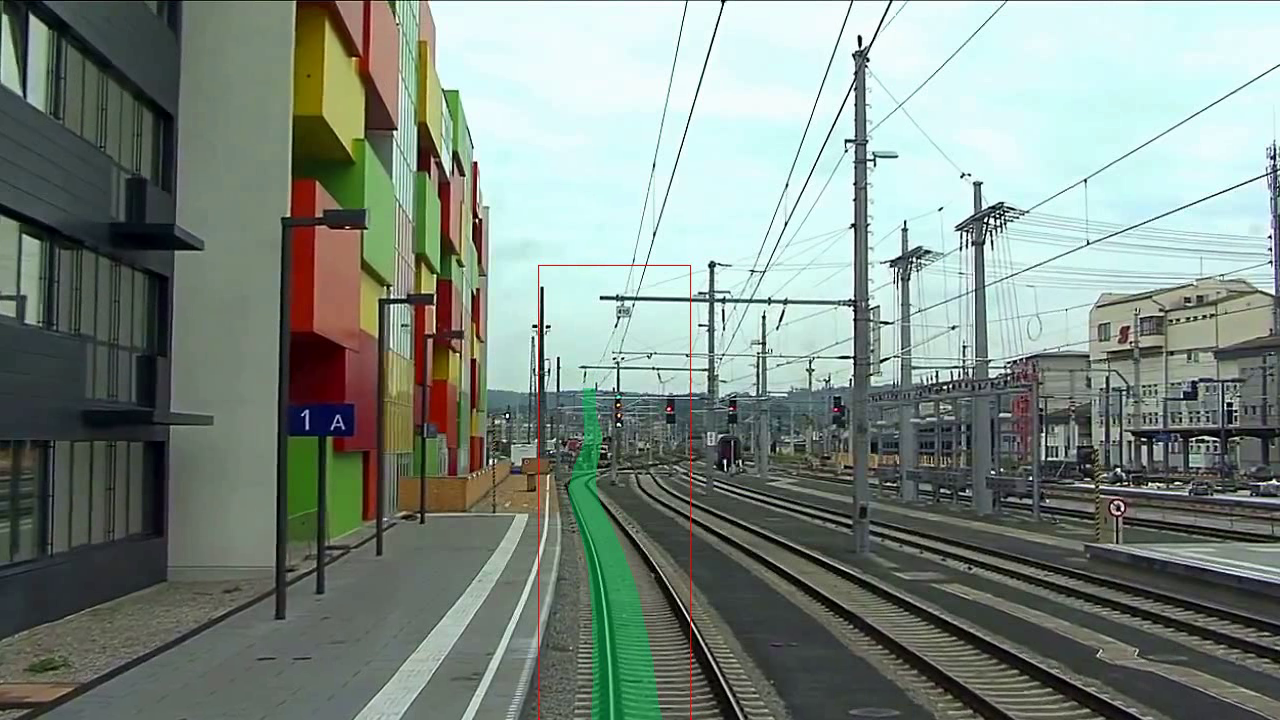
\includegraphics[width=\textwidth]{PICs/experiments/autocropExperiments/output_frames/frame_100.png}
    \end{minipage}
    \hfill
    \begin{minipage}{0.195\textwidth}
        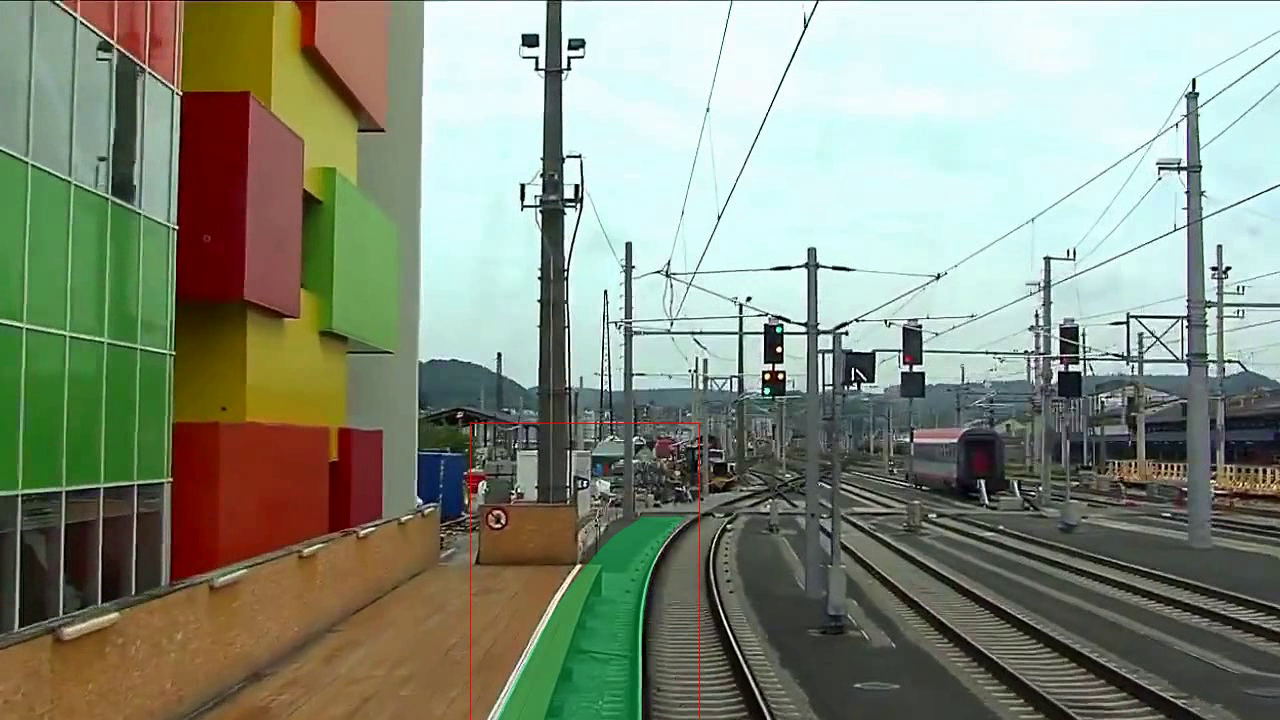
\includegraphics[width=\textwidth]{PICs/experiments/autocropExperiments/output_frames/frame_700.png}
    \end{minipage}
    \hfill
    \begin{minipage}{0.195\textwidth}
        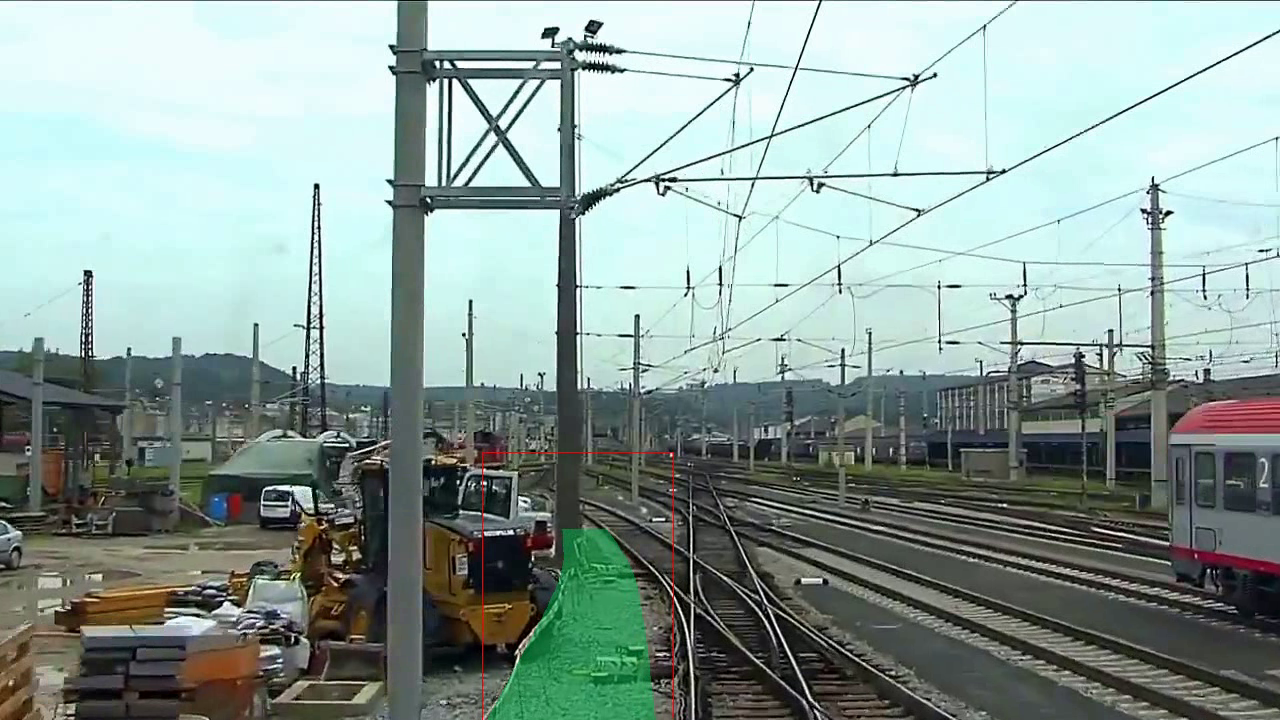
\includegraphics[width=\textwidth]{PICs/experiments/autocropExperiments/output_frames/frame_1000.png}
    \end{minipage}
    \hfill
    \begin{minipage}{0.195\textwidth}
        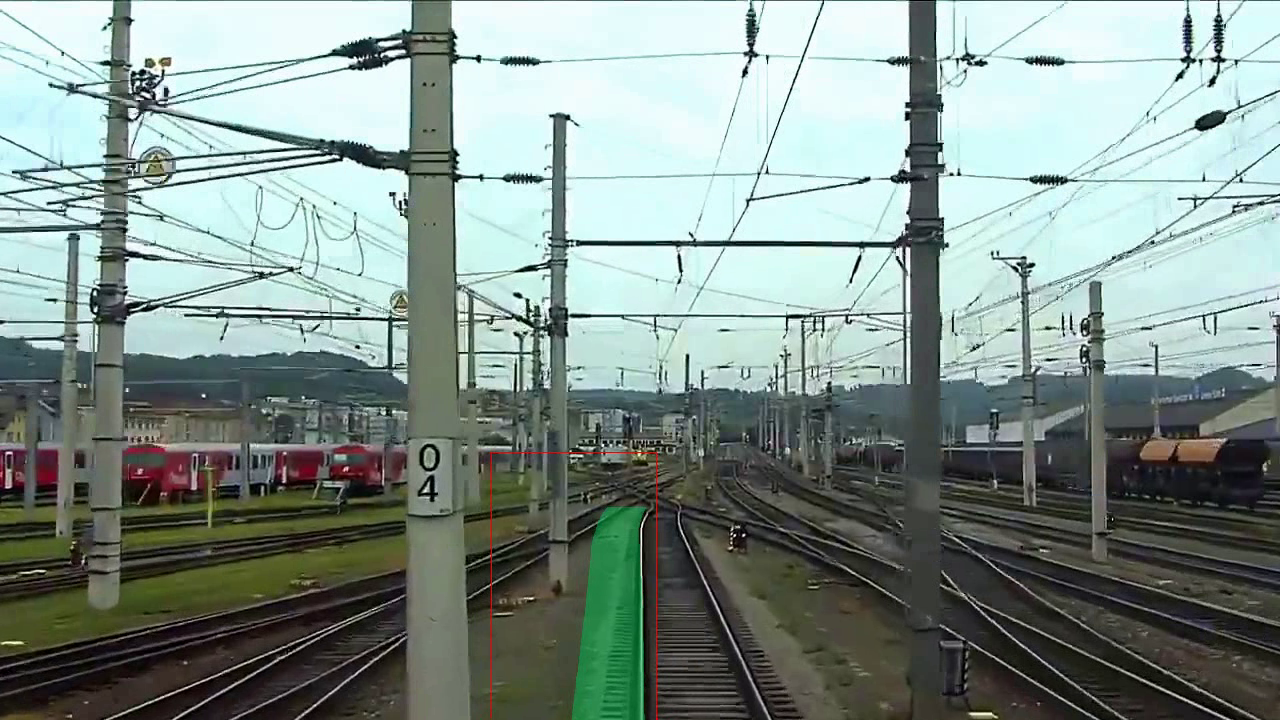
\includegraphics[width=\textwidth]{PICs/experiments/autocropExperiments/output_frames/frame_1600.png}
    \end{minipage}
    \hfill
    \begin{minipage}{0.195\textwidth}
        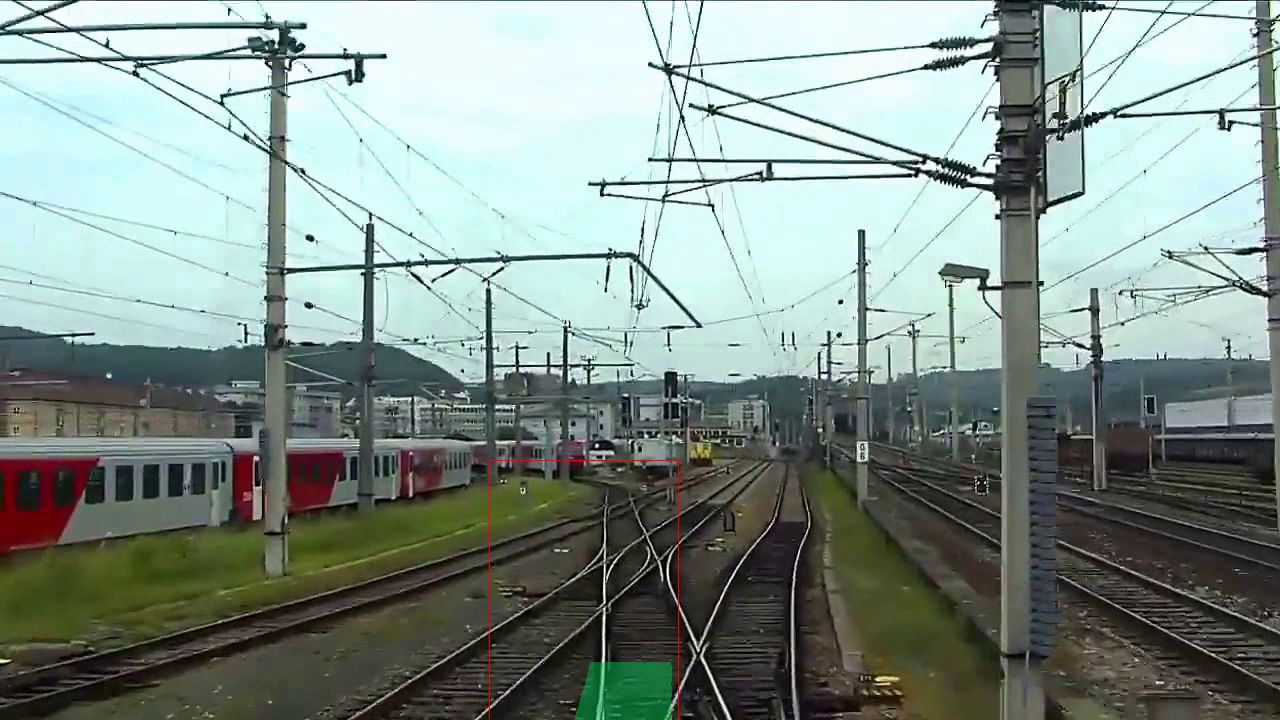
\includegraphics[width=\textwidth]{PICs/experiments/autocropExperiments/output_frames/frame_1900.png}
    \end{minipage}

    % Unteres Grid mit kleineren Bildern
    \begin{minipage}{0.195\textwidth}
        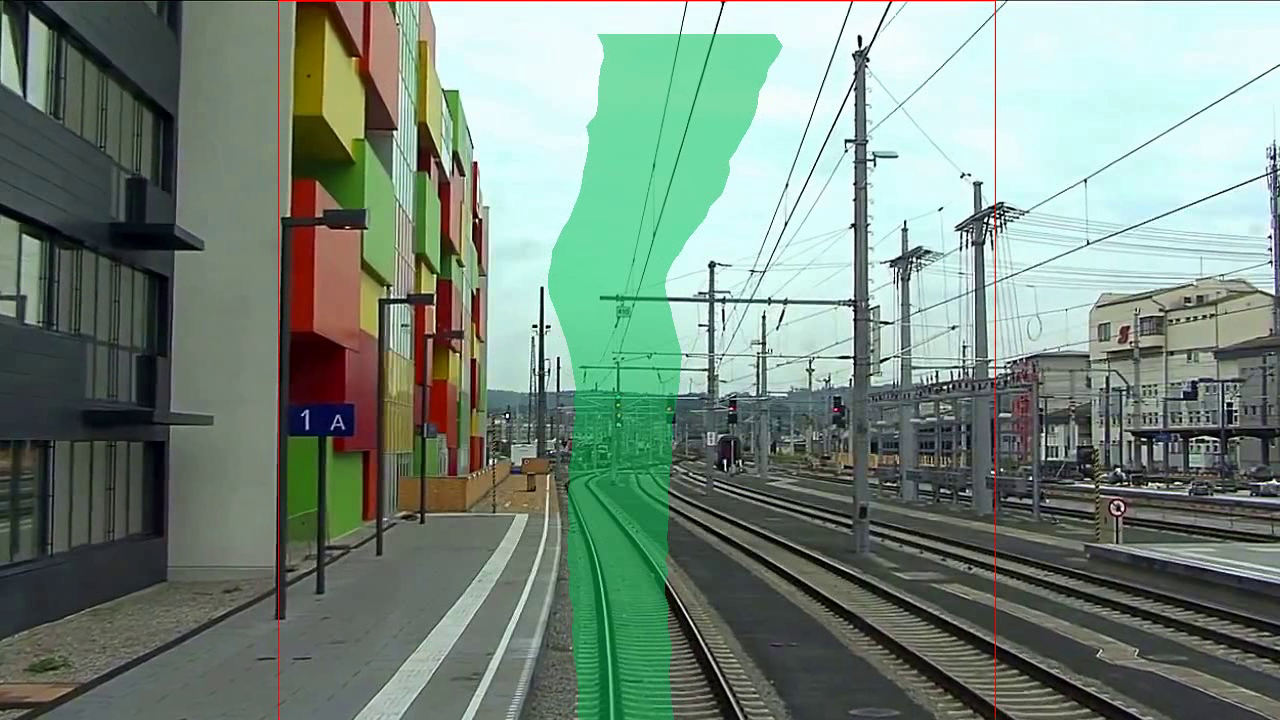
\includegraphics[width=\textwidth]{PICs/experiments/autocropExperiments/output_frames_improved/frame_100.png}
    \end{minipage}
    \hfill
    \begin{minipage}{0.195\textwidth}
        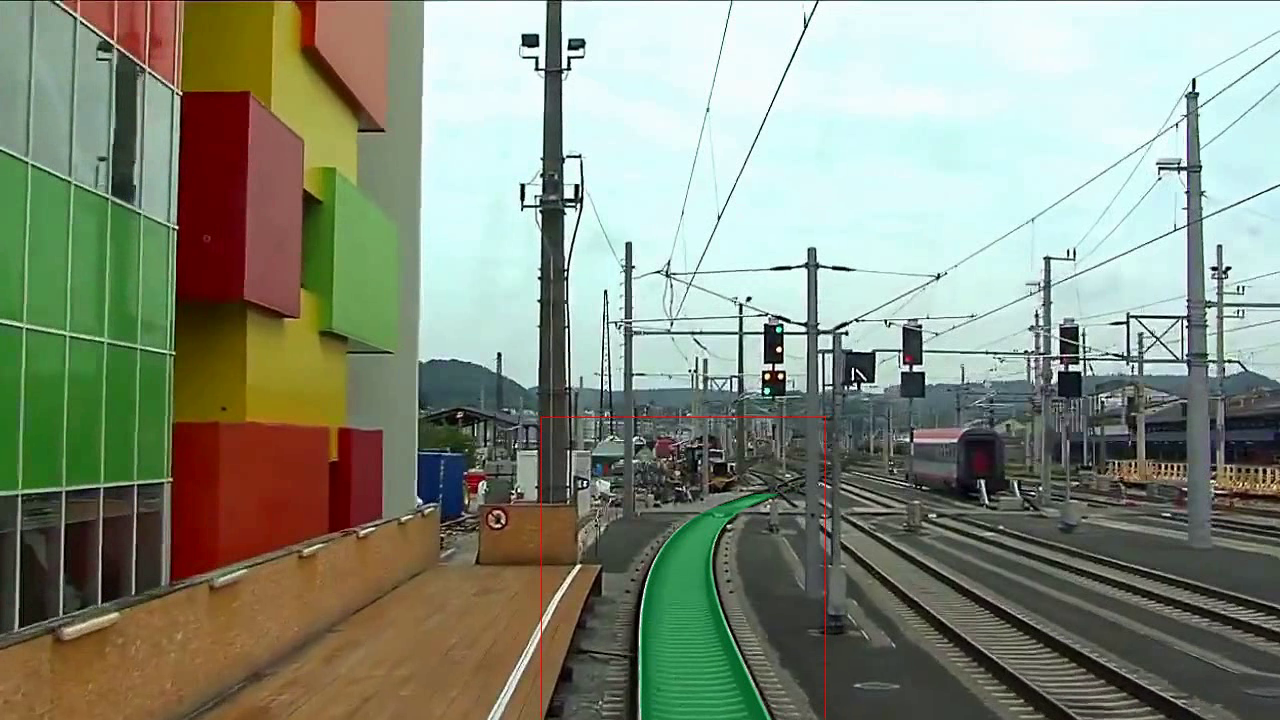
\includegraphics[width=\textwidth]{PICs/experiments/autocropExperiments/output_frames_improved/frame_700.png}
    \end{minipage}
    \hfill
    \begin{minipage}{0.195\textwidth}
        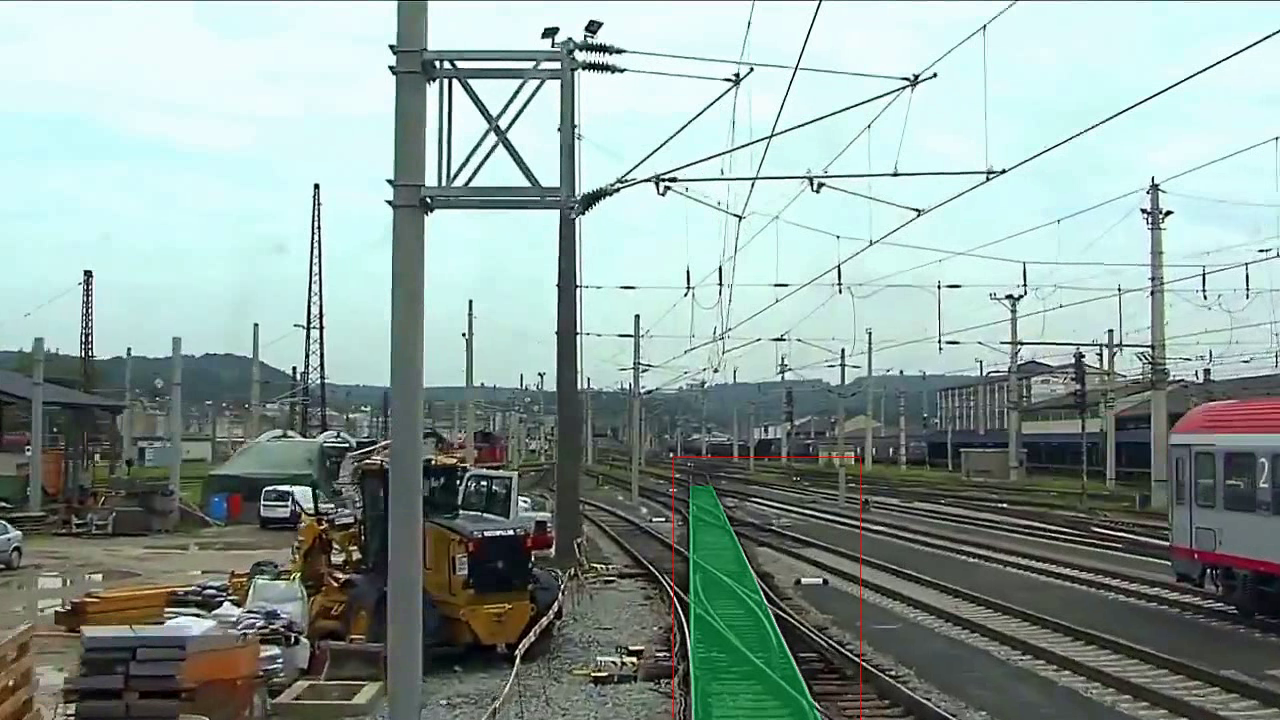
\includegraphics[width=\textwidth]{PICs/experiments/autocropExperiments/output_frames_improved/frame_1000.png}
    \end{minipage}
    \hfill
    \begin{minipage}{0.195\textwidth}
        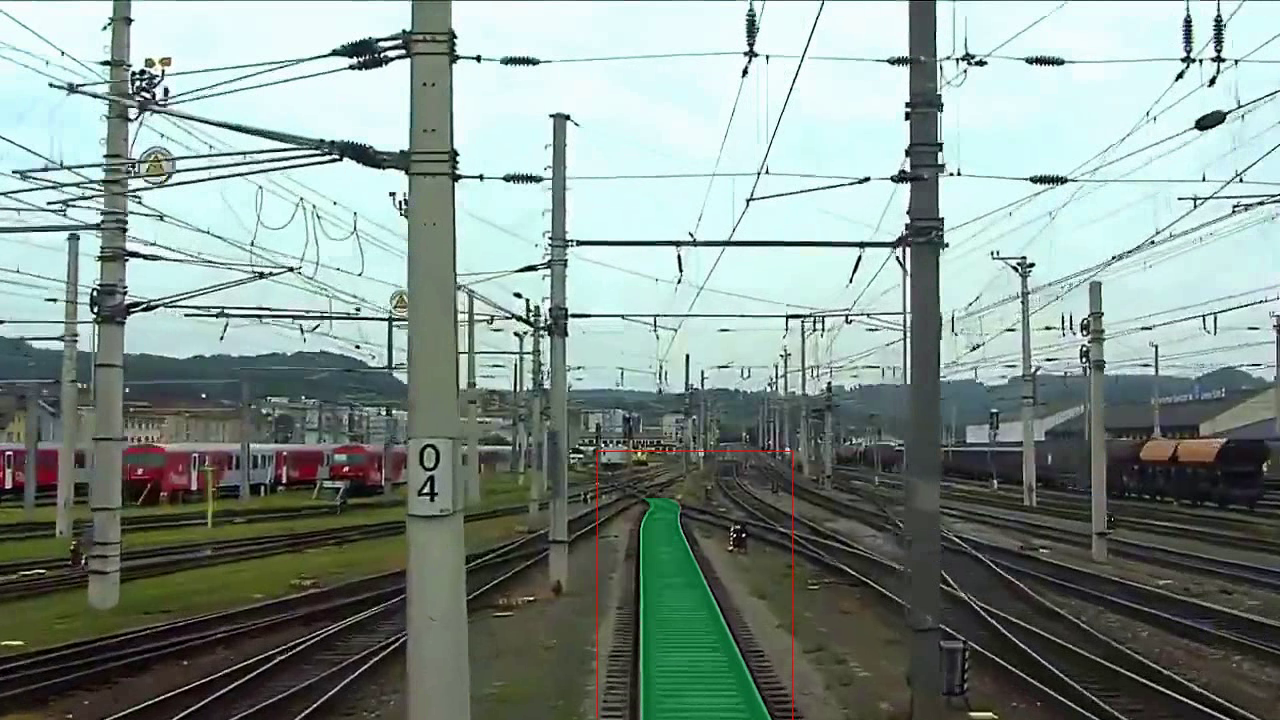
\includegraphics[width=\textwidth]{PICs/experiments/autocropExperiments/output_frames_improved/frame_1600.png}
    \end{minipage}
    \hfill
    \begin{minipage}{0.195\textwidth}
        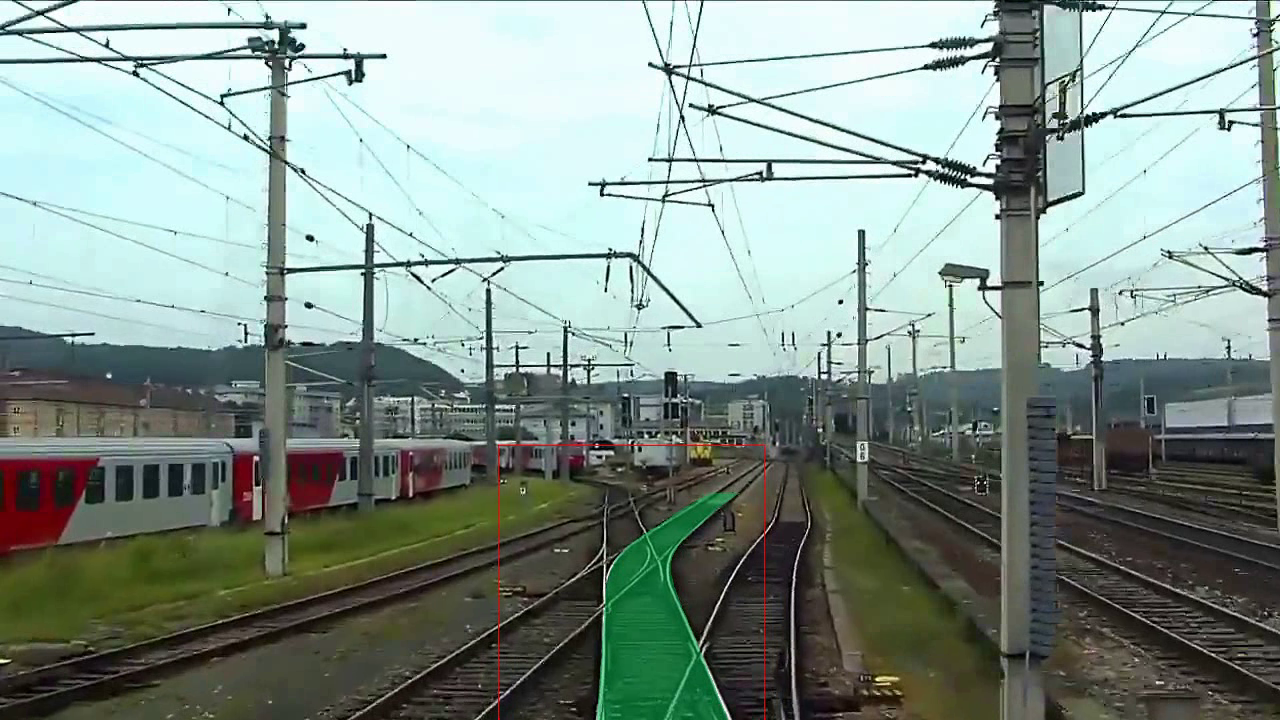
\includegraphics[width=\textwidth]{PICs/experiments/autocropExperiments/output_frames_improved/frame_1900.png}
    \end{minipage}

    % Vierte Reihe für die Zeitachse
    \begin{minipage}{1.0\textwidth}
        \centering
        \begin{tikzpicture}
            % Zeit "Time" über dem Pfeil links positionieren
            \node at (-7.5, 0.3) {time}; % Text "Time"
            \draw[-Stealth, thick] (-8, 0) -- (8, 0); % Pfeil von ganz links nach ganz rechts
        \end{tikzpicture}
    \end{minipage}

    % Beschriftung unter dem Grid
    \vspace{0.5cm}
    \caption{Comparison between the original and the adapted auto-crop including frames 100, 700, 1000, 1600, and 1900 of the evaluation video \cite{temporalDataset_youtube_video}.
    First row is the original auto-crop from \cite{tepNet2024} and the second row is the proposed one.}
    \label{fig:autocropVideoComparison}
\end{figure}

\begin{figure}[H]
    \centering
    \begin{subfigure}{\textwidth}
        \centering
        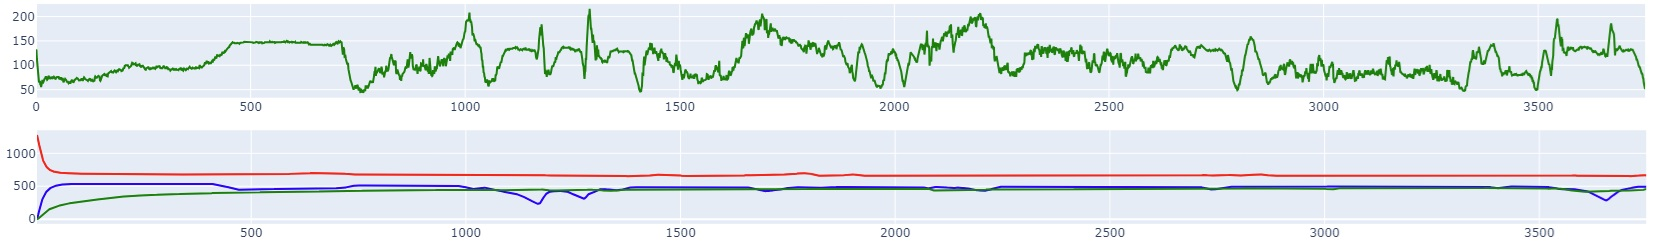
\includegraphics[width=\textwidth]{PICs/experiments/autocropExperiments/original.jpg} % erstes Bild
        \caption{Original auto-crop mechanism}
        \label{fig:autocropResultsTrends_a}
    \end{subfigure}
    %\hspace*{0.02\textwidth} % Abstand manuell steuern
    \begin{subfigure}{\textwidth}
        \centering
        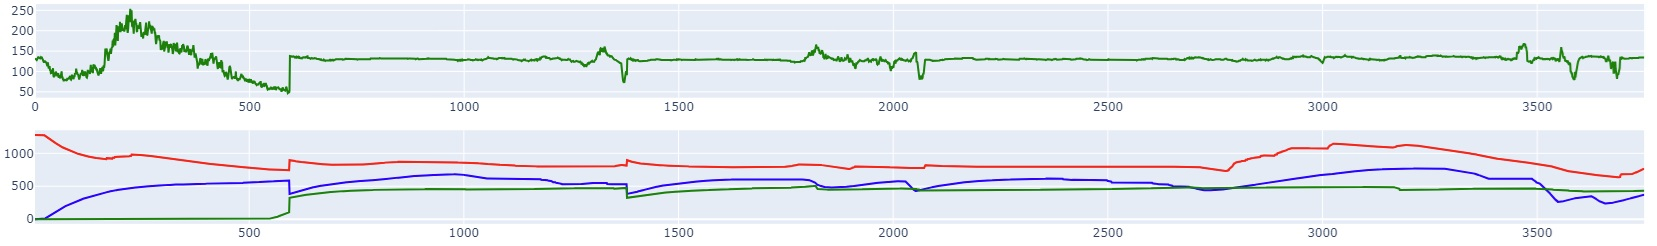
\includegraphics[width=\textwidth]{PICs/experiments/autocropExperiments/improved.jpg} % zweites Bild
        \caption{Adapted auto-crop mechanism (Version 2)}
        \label{fig:autocropResultsTrends_b}
    \end{subfigure}
    \caption{Tred of the evalutation video \cite{temporalDataset_youtube_video} shown in \autoref{fig:autocropVideoComparison}.
    The first and second graphs with a single green line show the rail width at the first anchor line.
    The second and fourth graph show crop coordinates (blue=left, red=right, green=top).
    Jumps in graphs from the adapted mechanism indicate resets, like the one at around frame 600.
    It also shows that with the original technique crop coords are stable and the prediction is not and the improved auto-crop reverses this relationship.}
    \label{fig:autocropResultsTrends}
\end{figure}


Models with a ResNet18 backbone show an additional behavior when uncertain.
The width of the predicted track becomes unstable, especially at the first few anchors.
This is because the camera is in a fixed position in this video \cite{temporalDataset_youtube_video}, and when correctly predicting the track, the width does not change at the bottom of the image.
Therefore, the track width at the first anchor line is a good indicator of uncertainty.
\autoref{fig:autocropVideoComparison} and \autoref{fig:autocropResultsTrends} show the evaluation of a model with the ResNet18 backbone on the evaluation video \cite{temporalDataset_youtube_video}.
\autoref{fig:autocropVideoComparison} shows the frames 100, 700, 1000, 1600, and 1900.
\autoref{fig:autocropResultsTrends} visualizes the trend of track width and crop coordinates.

As shown in frames 100, both models need time to find the right track.
The unstable rail width of both models also indicates this.
\autoref{fig:autocropResultsTrends_b} displays a jump of crop coords and rail width at around frame 600, indicating a reset.
After that, the adapted auto-crop mechanism proves to be correct and stable.
However, in the video with the original cropping mechanism, the crop converges to an area that does not include the rail.
Since the system does not include a reset rule, it cannot recover from the mistake at the start.
When comparing both techniques in a broader scope, the original cropping mechanism shows stable crop coordinates, but the prediction is often incorrect.
On the other hand, the adapted technique moves more freely and quickly adapts to challenging scenarios.
Consequently, the prediction becomes more stable, which is the desired output.